\PassOptionsToPackage{unicode=true}{hyperref} % options for packages loaded elsewhere
\PassOptionsToPackage{hyphens}{url}
%
\documentclass[14pt,ignorenonframetext,]{beamer}
\usepackage{pgfpages}
\setbeamertemplate{caption}[numbered]
\setbeamertemplate{caption label separator}{: }
\setbeamercolor{caption name}{fg=normal text.fg}
\beamertemplatenavigationsymbolsempty
\usepackage{lmodern}
\usepackage{amssymb,amsmath}
\usepackage{ifxetex,ifluatex}
\usepackage{fixltx2e} % provides \textsubscript
\ifnum 0\ifxetex 1\fi\ifluatex 1\fi=0 % if pdftex
  \usepackage[T1]{fontenc}
  \usepackage[utf8]{inputenc}
  \usepackage{textcomp} % provides euro and other symbols
\else % if luatex or xelatex
  \usepackage{unicode-math}
  \defaultfontfeatures{Ligatures=TeX,Scale=MatchLowercase}
\fi
\usetheme[]{metropolis}
% use upquote if available, for straight quotes in verbatim environments
\IfFileExists{upquote.sty}{\usepackage{upquote}}{}
% use microtype if available
\IfFileExists{microtype.sty}{%
\usepackage[]{microtype}
\UseMicrotypeSet[protrusion]{basicmath} % disable protrusion for tt fonts
}{}
\IfFileExists{parskip.sty}{%
\usepackage{parskip}
}{% else
\setlength{\parindent}{0pt}
\setlength{\parskip}{6pt plus 2pt minus 1pt}
}
\usepackage{hyperref}
\hypersetup{
            pdftitle={Feature-based time series analysis},
            pdfauthor={Rob J Hyndman},
            pdfborder={0 0 0},
            breaklinks=true}
\urlstyle{same}  % don't use monospace font for urls
\newif\ifbibliography
\usepackage{graphicx,grffile}
\makeatletter
\def\maxwidth{\ifdim\Gin@nat@width>\linewidth\linewidth\else\Gin@nat@width\fi}
\def\maxheight{\ifdim\Gin@nat@height>\textheight\textheight\else\Gin@nat@height\fi}
\makeatother
% Scale images if necessary, so that they will not overflow the page
% margins by default, and it is still possible to overwrite the defaults
% using explicit options in \includegraphics[width, height, ...]{}
\setkeys{Gin}{width=\maxwidth,height=\maxheight,keepaspectratio}
% Prevent slide breaks in the middle of a paragraph:
\widowpenalties 1 10000
\raggedbottom
\setbeamertemplate{part page}{
\centering
\begin{beamercolorbox}[sep=16pt,center]{part title}
  \usebeamerfont{part title}\insertpart\par
\end{beamercolorbox}
}
\setbeamertemplate{section page}{
\centering
\begin{beamercolorbox}[sep=12pt,center]{part title}
  \usebeamerfont{section title}\insertsection\par
\end{beamercolorbox}
}
\setbeamertemplate{subsection page}{
\centering
\begin{beamercolorbox}[sep=8pt,center]{part title}
  \usebeamerfont{subsection title}\insertsubsection\par
\end{beamercolorbox}
}
\AtBeginPart{
  \frame{\partpage}
}
\AtBeginSection{
  \ifbibliography
  \else
    \frame{\sectionpage}
  \fi
}
\AtBeginSubsection{
  \frame{\subsectionpage}
}
\setlength{\emergencystretch}{3em}  % prevent overfull lines
\providecommand{\tightlist}{%
  \setlength{\itemsep}{0pt}\setlength{\parskip}{0pt}}
\setcounter{secnumdepth}{0}

% set default figure placement to htbp
\makeatletter
\def\fps@figure{htbp}
\makeatother

\usepackage{MonashBlue}
\usepackage[lf,t]{carlito}
\graphicspath{{figs/}}
\usepackage{bm}
\def\full#1{\vspace*{0.2cm}\par\centerline{\includegraphics[height=8.1cm,width=12.8cm,keepaspectratio=true]{#1}}}

\def\Var{\text{Var}}

\setkeys{Gin}{width=11.7cm,height=8cm,keepaspectratio}

\title{Feature-based time series analysis}
\author{Rob J Hyndman}
\date{21 June 2018}

\begin{document}
\frame{\titlepage}

\hypertarget{m3-competition}{%
\section{M3 competition}\label{m3-competition}}

\begin{frame}{M3 competition}
\protect\hypertarget{m3-competition-1}{}

\full{M3paper}
\only<2>{
\placefig{1}{4}{height=3cm}{SMakridakis}
\placefig{8.5}{4}{height=3cm}{MHibon}}

\end{frame}

\begin{frame}{How to plot lots of time series?}
\protect\hypertarget{how-to-plot-lots-of-time-series}{}

\only<1>{\full{M3data1}}
\only<2>{\full{M3data2}}
\only<3>{\full{M3data3}}
\only<4>{\full{M3data4}}
\only<5>{\full{M3data5}}
\only<6>{\full{M3data10}}
\only<7>{\full{M3data20}}
\only<8>{\full{M3data30}}
\only<9>{\full{M3data40}}
\only<10>{\full{M3data50}}
\only<11>{\full{M3data100}}
\only<12>{\full{M3data200}}
\only<13>{\full{M3data500}}
\only<14>{\full{M3dataall}}

\end{frame}

\begin{frame}{Key idea}
\protect\hypertarget{key-idea}{}

\placefig{9.1}{.5}{width=3.6cm}{tukey}
\begin{textblock}{3}(9.7,5.4)\small\textit{John W Tukey}\end{textblock}
\begin{textblock}{8}(0.7,1.2)
\begin{alertblock}{Cognostics}
Computer-produced diagnostics\\ (Tukey and Tukey, 1985).
\end{alertblock}
\end{textblock}\pause
\vspace*{2.5cm}

\alert{Examples for time series}

\begin{itemize}
\tightlist
\item
  lag correlation
\item
  size and direction of trend
\item
  strength of seasonality
\item
  timing of peak seasonality
\item
  spectral entropy
\end{itemize}

\vspace*{0.3cm}
\begin{block}{}
Called ``features'' in the machine learning literature.
\end{block}

\end{frame}

\begin{frame}{An STL decomposition: N2096}
\protect\hypertarget{an-stl-decomposition-n2096}{}

\begin{alertblock}{}
\centerline{$Y_t = S_t + T_t + R_t$\qquad $S_{t}$ is periodic with mean 0}
\end{alertblock}

\includegraphics{fbtsa_files/figure-beamer/stl-1.pdf}

\end{frame}

\begin{frame}{Candidate features}
\protect\hypertarget{candidate-features}{}

\begin{block}{STL decomposition}
\centerline{$Y_t = S_t + T_t + R_t$}
\end{block}\pause\fontsize{13}{15}\sf

\begin{itemize}
\tightlist
\item
  Seasonal period
\item
  Autocorrelations of data (\(Y_1,\dots,Y_T\))
\item
  Autocorrelations of data (\(R_1,\dots,R_T\))
\item
  Strength of seasonality:
  \(\max\left(0,1 - \frac{\Var(R_t)}{\Var(Y_t-T_t)}\right)\)
\item
  Strength of trend:
  \(\max\left(0,1 - \frac{\Var(R_t)}{\Var(Y_t-S_t)}\right)\)
\item
  Spectral entropy:
  \(H = - \int_{-\pi}^{\pi} f_y(\lambda) \log f_y(\lambda) d\lambda\),
  where \(f_y(\lambda)\) is spectral density of
  \(Y_t\).\textbackslash{}newline Low values of \(H\) suggest a time
  series that is easier to forecast (more signal).
\item
  Optimal Box-Cox transformation of data
\end{itemize}

\end{frame}

\hypertarget{tsfeatures}{%
\section{tsfeatures}\label{tsfeatures}}

\begin{frame}{Hyndman, Wang and Laptev (ICDM 2015)}
\protect\hypertarget{hyndman-wang-and-laptev-icdm-2015}{}

\includegraphics{fbtsa_files/figure-beamer/yahoo2-1.pdf}

\end{frame}

\begin{frame}{Kang, Hyndman \& Smith-Miles (IJF 2017)}
\protect\hypertarget{kang-hyndman-smith-miles-ijf-2017}{}

\includegraphics{fbtsa_files/figure-beamer/ijf2017graphs-1.pdf}
\includegraphics{fbtsa_files/figure-beamer/ijf2017graphs-2.pdf}

\end{frame}

\hypertarget{irish-smart-metre-data}{%
\section{Irish smart metre data}\label{irish-smart-metre-data}}

\begin{frame}{Irish smart metre data}
\protect\hypertarget{irish-smart-metre-data-1}{}

\centerline{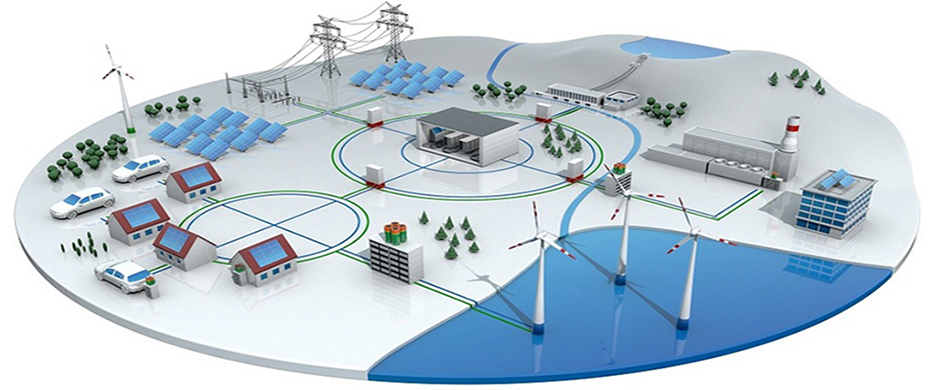
\includegraphics[width=1.18\linewidth]{SMARTGRID.jpg}}
  \vspace{-.85cm}
  \begin{flushright}
    { \tiny Figure: \url{http://solutions.3m.com}}
  \end{flushright}\vspace*{-0.4cm}\fontsize{12}{13}\sf

\begin{itemize}
\tightlist
\item
  500 households from smart metering trial
\item
  Electricity consumption at 30-minute intervals\newline between 14 July
  2009 and 31 December 2010
\item
  Heating/cooling energy usage excluded
\end{itemize}

\end{frame}

\begin{frame}{Irish smart metre data}
\protect\hypertarget{irish-smart-metre-data-2}{}

\includegraphics{fbtsa_files/figure-beamer/timeplot1-1.pdf}

\end{frame}

\begin{frame}{Irish smart metre data}
\protect\hypertarget{irish-smart-metre-data-3}{}

\includegraphics{fbtsa_files/figure-beamer/timeplot2-1.pdf}

\end{frame}

\begin{frame}{Irish smart metre data}
\protect\hypertarget{irish-smart-metre-data-4}{}

\includegraphics{fbtsa_files/figure-beamer/timeplot3-1.pdf}

\end{frame}

\hypertarget{quantiles-conditional-on-time-of-week}{%
\section{Quantiles conditional on time of
week}\label{quantiles-conditional-on-time-of-week}}

\begin{frame}{Quantiles conditional on time of week}
\protect\hypertarget{quantiles-conditional-on-time-of-week-1}{}

\fontsize{11}{13}\sf

\begin{itemize}
\tightlist
\item
  Compute sample quantiles at \(p=0.01,0.02,\dots, 0.99\) for each
  household and each half-hour of the week.
\item
  \(336\) probability distributions per household.
\end{itemize}

\includegraphics{fbtsa_files/figure-beamer/timeplot1repeat-1.pdf}

\end{frame}

\begin{frame}{Quantiles conditional on time of week}
\protect\hypertarget{quantiles-conditional-on-time-of-week-2}{}

\fontsize{11}{13}\sf

\begin{itemize}
\tightlist
\item
  Compute sample quantiles at \(p=0.01,0.02,\dots, 0.99\) for each
  household and each half-hour of the week.
\item
  \(336\) probability distributions per household.
\end{itemize}

\includegraphics{fbtsa_files/figure-beamer/qdemandplot1-1.pdf}

\end{frame}

\begin{frame}{Quantiles conditional on time of week}
\protect\hypertarget{quantiles-conditional-on-time-of-week-3}{}

\fontsize{11}{13}\sf

\begin{itemize}
\tightlist
\item
  Compute sample quantiles at \(p=0.01,0.02,\dots, 0.99\) for each
  household and each half-hour of the week.
\item
  \(336\) probability distributions per household.
\end{itemize}

\includegraphics{fbtsa_files/figure-beamer/timeplot2repeat-1.pdf}

\end{frame}

\begin{frame}{Quantiles conditional on time of week}
\protect\hypertarget{quantiles-conditional-on-time-of-week-4}{}

\fontsize{11}{13}\sf

\begin{itemize}
\tightlist
\item
  Compute sample quantiles at \(p=0.01,0.02,\dots, 0.99\) for each
  household and each half-hour of the week.
\item
  \(336\) probability distributions per household.
\end{itemize}

\includegraphics{fbtsa_files/figure-beamer/qdemandplot2-1.pdf}

\end{frame}

\begin{frame}{Quantiles conditional on time of week}
\protect\hypertarget{quantiles-conditional-on-time-of-week-5}{}

\fontsize{11}{13}\sf

\begin{itemize}
\tightlist
\item
  Compute sample quantiles at \(p=0.01,0.02,\dots, 0.99\) for each
  household and each half-hour of the week.
\item
  \(336\) probability distributions per household.
\end{itemize}

\includegraphics{fbtsa_files/figure-beamer/timeplot3repeat-1.pdf}

\end{frame}

\begin{frame}{Quantiles conditional on time of week}
\protect\hypertarget{quantiles-conditional-on-time-of-week-6}{}

\fontsize{11}{13}\sf

\begin{itemize}
\tightlist
\item
  Compute sample quantiles at \(p=0.01,0.02,\dots, 0.99\) for each
  household and each half-hour of the week.
\item
  \(336\) probability distributions per household.
\end{itemize}

\includegraphics{fbtsa_files/figure-beamer/qdemandplot3-1.pdf}

\end{frame}

\begin{frame}{Quantiles conditional on time of week}
\protect\hypertarget{quantiles-conditional-on-time-of-week-7}{}

\fontsize{12}{13}\sf

\centerline{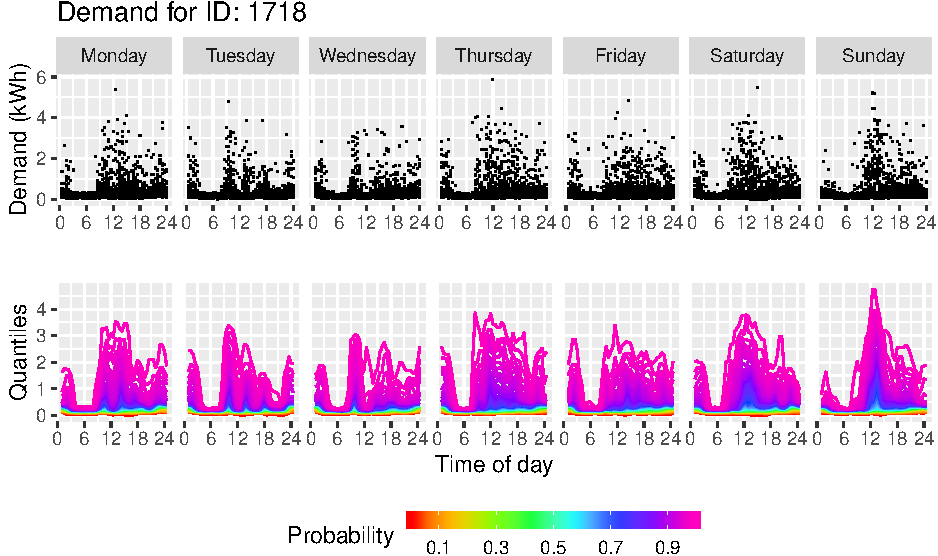
\includegraphics[width=9.8cm]{quantileplot}}

\begin{itemize}[<+->]
\tightlist
\item
  Sample quantiles better than kernel density estimate:

  \begin{itemize}
  \item presence of zeros
  \item non-negative support
  \item high skewness
  \end{itemize}
\item
  Avoids missing data issues and variation in series length
\item
  Avoids timing of household events, holidays, etc.
\item
  Allows clustering of households based on probabilistic behaviour
  rather than coincident behaviour.
\item
  Allows identification of anomalous households.
\item
  Allows estimation of typical household behaviour.
\end{itemize}

\end{frame}

\hypertarget{finding-typical-and-unusual-households}{%
\section{Finding typical and unusual
households}\label{finding-typical-and-unusual-households}}

\begin{frame}{Pairwise distances}
\protect\hypertarget{pairwise-distances}{}

\placefig{0.1}{1.5}{width=5.5cm, height=1.8cm, keepaspectratio=false}{timeplot}
\placefig{7.2}{1.5}{width=5.5cm, height=1.8cm, keepaspectratio=false}{quantileplot}
\begin{textblock}{3}(5.7,2.2)\LARGE
$\longrightarrow$
\end{textblock}
\vspace*{.9cm}\fontsize{13}{15}\sf

\begin{itemize}
\item
  The time series of \(535\times48\) observations per household is
  mapped to a set of \(7\times48\times99\) quantiles giving a bivariate
  surface for each household.
\item
  Can we compute pairwise distances between all households?
\end{itemize}

\placefig{0.1}{7.5}{width=5.5cm, height=1.8cm, keepaspectratio=false}{quantileplot}
\placefig{7.2}{7.5}{width=5.5cm, height=1.8cm, keepaspectratio=false}{quantile2plot}
\begin{textblock}{1.48}(5.65,8.2)
$\leftarrow\hfill~?\hfill\rightarrow$\\\fontsize{11}{12}\sf
\hfill Distance \hfill
\end{textblock}

\end{frame}

\begin{frame}{Jensen-Shannon distances}
\protect\hypertarget{jensen-shannon-distances}{}

\begin{block}{Kullback-Leibler divergence between two densities}
$$D(p,q) = \int_{\infty}^\infty p(x) \log \frac{p(x)}{q(x)} dx$$
\vspace*{-0.2cm}\pause

Not symmetric: $D(p,q) \neq D(q,p)$
\end{block}
\pause

\begin{block}{Jensen-Shannon distance between two densities}
$$\text{JS}(p,q) =  [ D(p,r) +  D(q,r)] / 2\qquad\text{where~~}
r = (p+q)/2$$
\end{block}
\pause

\begin{block}{Distance between two households}
$$\Delta_{ij} = \sum_{t=1}^{7\times 48} \text{JS}(p_t,q_t)$$
\end{block}

\end{frame}

\begin{frame}{Kernel matrix and density ranking}
\protect\hypertarget{kernel-matrix-and-density-ranking}{}

\begin{block}{Similarity between two households}
$$
  w_{ij} = \exp(-\Delta_{ij}^2/h^2).
$$
\end{block}\pause

Row sums of the kernel matrix gives a scaled kernel density estimate of
households:

\begin{block}{}
$$  \hat{f}_i = \sum_{j=1}^n w_{ij}$$
\end{block}

\begin{itemize}
\tightlist
\item
  \(h\) is bandwidth in Gaussian kernel.
\item
  Households can be ranked by density values.
\end{itemize}

\end{frame}

\begin{frame}{Typical households}
\protect\hypertarget{typical-households}{}

\includegraphics{fbtsa_files/figure-beamer/typical-1.pdf}

\end{frame}

\begin{frame}{Typical households}
\protect\hypertarget{typical-households-1}{}

\includegraphics{fbtsa_files/figure-beamer/mode2-1.pdf}

\end{frame}

\begin{frame}{Typical households}
\protect\hypertarget{typical-households-2}{}

\includegraphics{fbtsa_files/figure-beamer/mode3-1.pdf}

\end{frame}

\begin{frame}{Anomalous households}
\protect\hypertarget{anomalous-households}{}

\includegraphics{fbtsa_files/figure-beamer/outlier1-1.pdf}

\end{frame}

\begin{frame}{Anomalous households}
\protect\hypertarget{anomalous-households-1}{}

\includegraphics{fbtsa_files/figure-beamer/outlier2-1.pdf}

\end{frame}

\begin{frame}{Anomalous households}
\protect\hypertarget{anomalous-households-2}{}

\includegraphics{fbtsa_files/figure-beamer/outlier3-1.pdf}

\end{frame}

\hypertarget{visualization-via-embedding}{%
\section{Visualization via
embedding}\label{visualization-via-embedding}}

\begin{frame}{Laplacian eigenmaps}
\protect\hypertarget{laplacian-eigenmaps}{}

\fontsize{13}{15}\sf

\begin{itemize}[<+->]
\tightlist
\item
  \textbf{Idea:} Embed conditional densities in a 2d space where the
  distances are preserved ``as far as possible''.
\item
  \begin{align*}
  \\[-1.36cm]
  \text{Let}\quad
  \bm{W} &=[w_{ij}] &&\text{~~ where~}w_{ij} = \exp(-\Delta_{ij}^2/h^2).\\
  \bm{D} &= \text{diag}(\hat{f}_i) &&\text{~~ where~}\hat{f}_i = \sum_{j=1}^n w_{ij}\\
  \bm{L} &=\bm{D}-\bm{W} &&\text{~~ (the Laplacian matrix).}\hspace{5cm}
  \end{align*}
\item
  Solve generalized eigenvector problem:
  \(\bm{L}\bm{e} = \lambda \bm{D}\bm{e}\).
\item
  Let \(\bm{e}_k\) be eigenvector corresponding to \(k\)th
  \emph{smallest} eigenvalue.
\item
  Then \(\bm{e}_2\) and \(\bm{e}_3\) create an embedding of households
  in 2d space.
\end{itemize}

\end{frame}

\begin{frame}{Key property of Laplacian embedding}
\protect\hypertarget{key-property-of-laplacian-embedding}{}

Let \(y_i = (e_{2,i},e_{3,i})\) be the embedded point corresponding to
household \(i\).

\begin{block}{}
Then the Laplacian eigenmap minimizes
$$
  \sum_{ij} w_{ij}(y_i-y_j)^2 = \bm{y}'\bm{L}\bm{y} \qquad\text{such that}\quad
\bm{y}'\bm{D}\bm{y}=1.
$$
\end{block}\pause

\begin{itemize}[<+->]
\tightlist
\item
  the most similar points are as close as possible.
\item
  First eigenvalue is 0 due to translation invariance.
\item
  Equivalent to optimal embedding using Laplace-Beltrami operator on
  manifolds.
\end{itemize}

\end{frame}

\begin{frame}{Outliers computed in embedded space:}
\protect\hypertarget{outliers-computed-in-embedded-space}{}

\end{frame}

\hypertarget{features-and-limitations}{%
\section{Features and limitations}\label{features-and-limitations}}

\begin{frame}{Features and limitations}
\protect\hypertarget{features-and-limitations-1}{}

\fontsize{12}{13}\sf

\begin{block}{Features of approach}
\begin{itemize}
 \item Converting time series to quantile surfaces conditional on time of week.
 \item Using pairwise distances between households
 \item Using kernel matrices for density ranking, embedding and clustering
\end{itemize}
\end{block}\pause

\textbf{Unresolved issues}

\begin{itemize}
\tightlist
\item
  Need to select the bandwidth \(h\) in constructing the similarity
  matrix.
\item
  Two different uses of bandwidth: density-ranking, embedding. Different
  bandwidth in each case?
\item
  The use of pairwise distances makes it hard to scale this algorithm.
\end{itemize}

\end{frame}

\end{document}
